\chapter{Analysis of correlated SiPM noise}
\label{ch:anal}

In the previous chapters we studied the sources of noise in the procedure to
identify and measure a single signal. However the photodetector itself produces
pulses which are not due to a detected photon. There are two kinds of these:
pulses which are produced independently of incident light, and pulses which are
produced by another pulse. The latter case is called \emph{correlated noise}.

We will give a brief explanation and classification of the SiPM noise and then
analyze it on a specific tile with LNGS laser data. We will see that we can
reliably measure only the correlated noise, hence the chapter title.

There are two goals in characterizing the SiPM noise. First, a quantitative
model of the noise is needed for the DarkSide20k simulation, and we will
provide an estimate of the parameters for a recent new production of SiPMs.
Second, our ``direct'' analysis method that looks at each single pulse in a
complete recorded finely-sampled waveform provides a cross-check for more
indirect methods that will be employed online in the VETO system which has less
powerful readout electronics.

\marginpar{I should add some reference for charge integration methods. Maybe
the article where I found the Borel the first time, \cite{chmill2017}. I may
do this in the local conclusions.}

\section{Theory}

\marginpar{In chapter~\ref{ch:snr} I will add a qualitative description that
can be deduced from the 2d histogram without previous knowledge apart from the
acquisition setup (the laser position). Just as an epistemic exercise. I must
also add the definition of PE.}

In \autoref{ch:snr} we briefly introduced the Silicon Photomultiplier (SiPM).
We will now give a more detailed explanation, mainly following
\cite[ch.~3]{savarese2018}. For a general introduction to semiconductor
detectors (but not the SiPM), see \cite[ch.~11]{knoll2010}.

The difference between a SiPM and older kinds of semiconductor detectors is
that the SiPM has a binary response: the amplitude of the output is not
proportional to the energy released by the detected particle. In this sense
they are analogous to Photomultiplier Tubes (PMTs), because they are designed
to detect just the presence of a photon with high efficiency ($\sim\SI{50}\%$).

A SiPM is composed by a grid of \emph{cells}. The cells are Single Photon
Avalanche Photodiodes (SPADs). A SPAD is a photodiode operated in reverse bias
above its breakdown voltage in series with a \emph{quenching resistor}. Since
the bias is above breakdown, if a current starts in the photodiode it will be
self sustaining and would normally destroy the diode. The resistor in series
lowers the potential difference on the diode when a current flows through it,
stopping the current because the diode goes below breakdown, so the output
pulse will have duration and amplitude uniquely determined by the resistor and
the capacitance of the diode junction, independently of the initial release of
energy that triggered the current.

The output from all the cells is summed analogically, so if multiple cells are
triggered simultaneously, the amplitude of the output pulse is discretized and
proportional to the number of fired cells. As we already said in
\autoref{ch:snr}, we will use the term ``PE'', standing for ``photoelectrons'',
as a unit when indicating the number of cells corresponding to a pulse.

\subsection{SiPM noise}

The initial creation of an electron-hole pair that starts the avalanche in the
photodiode can either be caused by an absorbed photon or by a thermal
fluctuation. The latter case happens randomly with fixed probability, and the
resulting rate of random pulses is called \emph{dark count rate}, where
``dark'' stands for the fact that this amounts to the total rate of pulses when
the photodiode is kept isolated from light.

The last sentence is actually not accurate because a ``primary'' pulse, either
a dark count or a photon, by various mechanisms can induce other pulses, that
can themselves recursively produce tertiary pulses in the same way. The four
ways in the proliferation of pulses are (see \autoref{fig:sipmnoise}):

\begin{description}

    \item[Afterpulses] During the avalanche, charge carriers can remain trapped
    into impurities and imperfections of the crystal. They are released
    afterwards at random, starting another avalanche in the same cell.
    
    \item[Direct cross talk (DiCT)] A photon emitted by an avalanche can
    trigger a nearby cell.
    
    \item[Delayed cross talk (DeCT)] Instead of hitting directly another cell,
    the photon can be absorbed in the shared crystal substrate and generate
    a hole that travels up until it passes through a cell and triggers it.
    
    \item[Delayed afterpulse] In the latter case, if the hole hits the
    originating cell, we call it delayed afterpulse instead of DeCT.

\end{description}

\begin{figure}
    
    \centering
    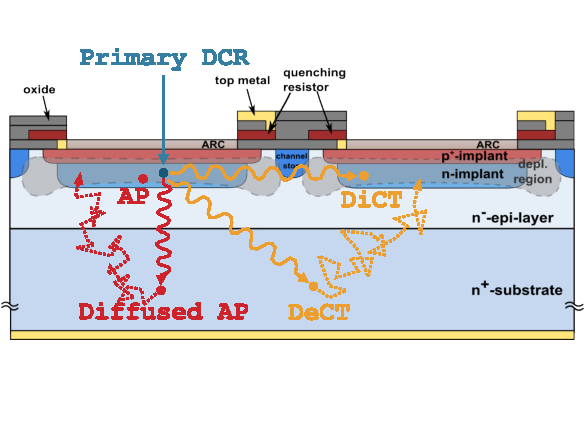
\includegraphics[width=0.85\textwidth]{sipmnoise}
    
    \caption{\label{fig:sipmnoise} Schematic of SiPM noises overlaid on the
    cross section of the device: AP (afterpulse), DiCT (direct cross talk),
    DeCT (delayed cross talk). From \cite[53]{savarese2018}.}
    
\end{figure}

The cells are less than \SI1{mm} wide, so the DiCT pulse starts within \SI1{ps}
of the originating pulse, while as we saw in \autoref{ch:snr} even just the
peak of the pulse lasts $\sim\SI{10}{ns}$. This means that the effect of the
DiCT is multiplying the height of the pulse by an integer factor, because the
overlapping pulses are well aligned. Afterpulses and DeCT, instead, can arrive
with a significative delay, and thus can be distinguished from the originating
pulse.

The reason why we classify separately the delayed pulses, instead of having an
overarching category of ``delayed noise'', is that afterpulses have a different
amplitude. The shape of the pulse is a sharp peak followed by an exponentially
decaying tail. This tail is due to the capacitance of the reverse-biased
junction that recharges through the quenching resistor after being discharged
inside the diode by the avalanche. A pulse generated by the same cell before
the recharge is complete can only use up the charge present in that moment.
Delayed cross talk, instead, has full amplitude because it involves a different
cell. See \autoref{fig:sipmnoiseampl}.

\begin{figure}
    
    \centering
    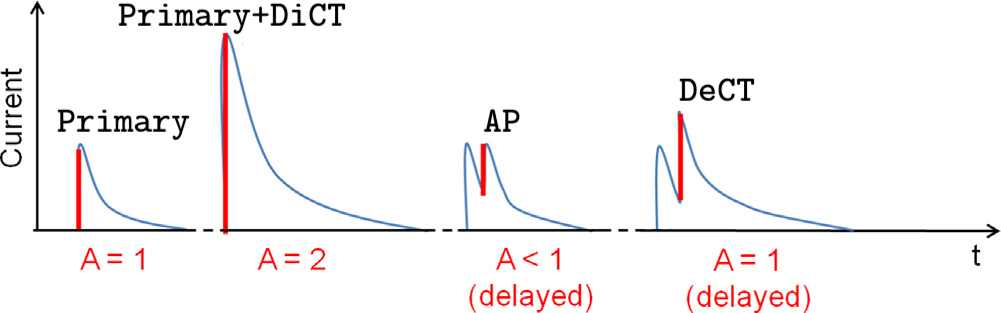
\includegraphics[width=0.85\textwidth]{sipmnoiseampl}
    
    \caption{\label{fig:sipmnoiseampl} Schematic of noise pulses. From
    \cite[4]{nagy2014}.}
    
\end{figure}

\subsection{DiCT model}

As we said, noise pulses can themselves produce other noise pulses as well. We
can imagine quite complicated interactions, for example: a DiCT induces a DeCT
on the original cell, thus producing a ``secondary'' delayed afterpulse. Or a
DiCT induces an afterpulse that induces a DiCT on the originating cell, again
with an afterpulse as final outcome. If the probabilities involved are small
enough, we should get by with the following simplifying assumption: that for
each pulse, the DiCT involves new cells that were not previously involved in
the chain, and the distribution of the number of DiCT at each step is fixed.

For the distribution to use for the generation model of DiCT, we follow
\cite{vinogradov2012}. Even when multiple DiCT steps are chained, the combined
delay is very small compared to the duration of the pulse, so the overall
effect of the complete DiCT ``tree'' is still to multiply the amplitude of the
first pulse. This means that at the end we just need to know the distribution
of the total number of consecutive DiCT.

For the single DiCT step, we consider two distributions: Bernoulli and Poisson.
In the first case we assume that a cell can induce a DiCT in at most just
another cell. In the second, we assume that there is a infinite population of
other cells, each with a fixed probability to be triggered. Clearly these two
cases are ``opposite'' approximations. In the first case, the distribution of
the total number of PE $k$ is Geometric. If $p$ is the probability of
generating a DiCT at each step, the distribution is
%
\begin{equation}
    P_G(k;p) = p^{k-1}(1-p), \quad k \ge 1, \quad p \in [0,1).
    \label{eq:geometric}
\end{equation}
%
Note that the conventional parametrization of the Geometric distribution is
different, with $p$ and $1 - p$ interchanged. We use this formulation because
it is more intuitively comparable with the other case. If the branching
distribution is Poisson with mean $\mu_B$, the total distribution is the Borel,
%
\begin{equation}
    P_B(k;\mu_B) = e^{-k\mu_B} \frac {(k\mu_B)^{k-1}} {k!},
    \quad k \ge 1, \quad \mu_B \in [0,1).
    \label{eq:borel}
\end{equation}
%
If it was $\mu_B \ge 1$, $k$ would diverge with nonzero probability.

The formula for the mean is formally the same for the two distributions,
%
\begin{equation}
    E[k] = \frac 1 {1 - p} = \frac 1 {1 - \mu_B},
\end{equation}
%
thus, since the interesting quantity is the amount of excess pulses due to
noise, it makes sense to compare the two distributions when $p = \mu_B$. We
make such comparison in \autoref{fig:geomborel} for $p = \mu_B = 0.5$. We note
that the Borel distribution has higher probability on the no-DiCT case, and at
the same time a fatter tail, while being lower in the few-DiCT cases.

\begin{figure}
    
    \hspace{-0.10\textwidth}
    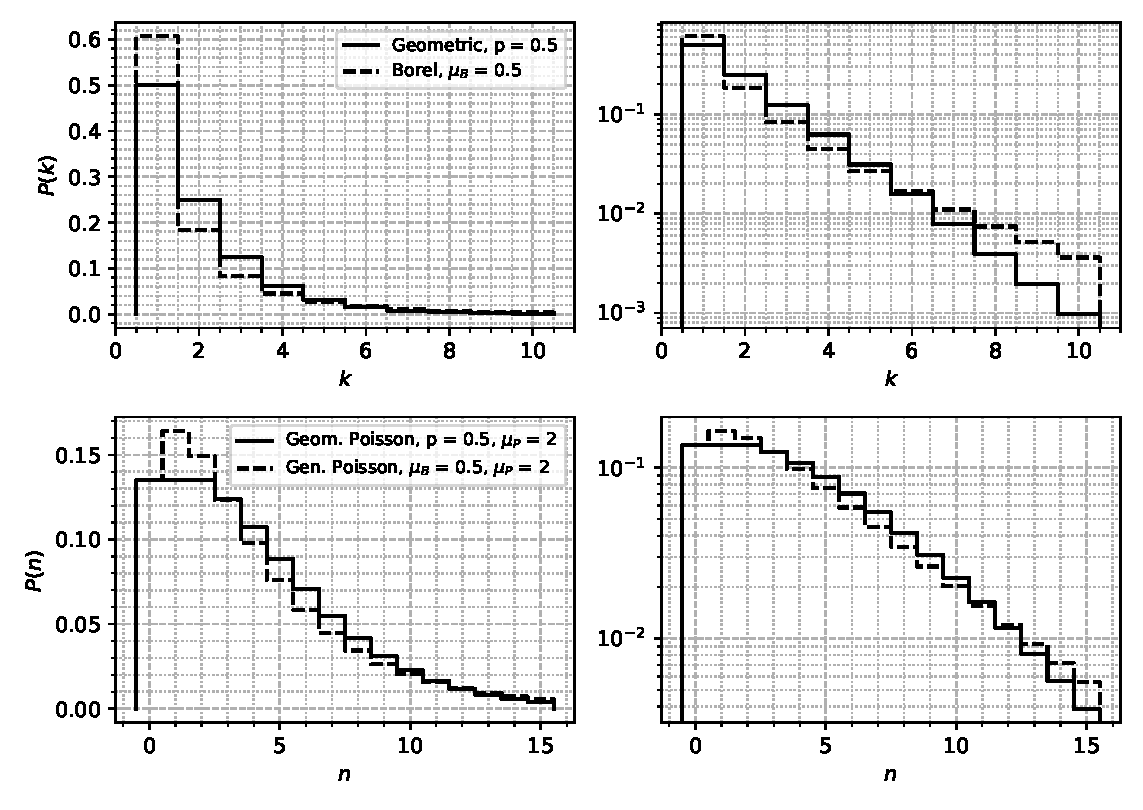
\includegraphics[width=1.19\textwidth]{figgeomborel}

    \figcaption{geomborel}{Top panels: comparison of the geometric and Borel
    distributions (Equations~\ref{eq:geometric} and~\ref{eq:borel}), used for
    the total number of pulses in the DiCT tree, including the initial pulse.
    Bottom panels: geometric and generalized Poisson
    (Equations~\ref{eq:geompoisson} and~\ref{eq:genpoisson}), for the total
    number of PE when the number of initial pulses is Poisson distributed. The
    right panels are the same plots on the left in logarithmic scale.}
    
\end{figure}

Since we use laser data, there are multiple photons hitting the SiPM. The light
is diffused before reaching the photodetector (see \autoref{ch:data}), so we
expect at most one photon per cell, and thus a Poisson distribution for the
initial number of fired cells. So for the analysis we will need the
distribution of the total number of PE $n \ge 0$ for an initial
Poisson-distributed number of cells, each with its DiCT tree.

For the geometric model, the resulting distribution is called geometric Poisson
or Pólya-Aeppli. Let $\mu_P$ be the initial Poisson mean. The probability mass
function $P_{GP}$ can be computed with this recursion \cite[5]{nuel2008}:
%
\begin{align}
    P_n &\equiv P_{GP}(n;\mu_P,p), \\
    z &\equiv \mu_P \frac{1-p}p, \\
    P_0 &= e^{-\mu_P}, \\
    P_1 &= e^{-\mu_P} zp, \\
    P_n &= \frac{2n - 2 + z}n p P_{n-1} + \frac{2-n}n p^2 P_{n-2}.
    \label{eq:geompoisson}
\end{align}

For the Borel model, the distribution is the generalized Poisson:
%
\begin{equation}
    P_{BP}(n;\mu_P,\mu_B)
    = e^{-(\mu_P + n\mu_B)} \frac {\mu_P(\mu_P + n\mu_B)^{n-1}} {n!}.
    \label{eq:genpoisson}
\end{equation}

The means of the two distributions are, unsurprisingly, $\mu_P/(1-p)$ and
$\mu_P/(1-\mu_B)$. Note that for $n = 0$ the probabilities are equal, since
of course the cross talk does not affect the zero initial pulses case.

The referenced article finds a much better agreement with the Borel model when
looking at the tails of the PE distribution for DiCT only
\cite[p.~3~fig.~1]{vinogradov2012}, while it does not find a visible difference
for the Poisson+DiCT distribution with $\text{PE} \le 11$
\cite[p.~4~fig.~2]{vinogradov2012}.

\subsection{Afterpulse model}

For the afterpulses we have to model not just the number of pulses, but also
their temporal distribution and amplitude.

Afterpulses are produced by carriers trapped during the avalanche that get
released afterwards. Following \cite[1]{nagy2014}, we claim that this fact has
been proven by \cite{cova1991}, although by reading the latter article we feel
that their report is a bit too synthetic.

The release of trapped carriers is a thermodynamical process regulated by the
potential difference that the carriers must overcome to jump out of their
traps. This means that it also depends on the external bias. If there was only
one kind of trap, the temporal distribution of carrier releasing would be
exponential. However we expect to have various possible trapping energy levels,
so the distribution is in general a mixture of exponentials.

The released carriers also have a non-unitary probability of generating an
avalanche. This probability also depends on the electric field and thus on the
bias, like the release probability. The bias in turn depends on the recharge
state of the cell, thus deforming the exponential distribution for low delays.

While \cite[2]{nagy2014} tries to keep into account this deviation by
multiplying the afterpulse temporal distribution with the fraction of recovered
charge
%
\begin{equation}
    1 - \exp\left(-\frac{t}{\tau_\text{rec}}\right),
    \label{eq:recfactor}
\end{equation}
%
where $\tau_\text{rec}$ is the exponential scale of the pulse shape tail,
\cite[4]{garutti2014} goes straight with pure exponentials. However, we notice
from \cite[p.~5~fig.~11]{nagy2014}, reported here in \autoref{fig:nagyap}, that
they do not actually have data at low delays to test the accuracy of their
model, since the relatively high threshold they use for peak finding truncates
the afterpulse distribution at $\approx\SI{80}{ns}$. Even though the recharge
time is $\tau_\text{rec} = \SI{207}{ns}$, thus making the correction term
\eqref{eq:recfactor} significative even above the temporal cut, by looking at
the plotted histogram we think that a vanilla exponential with a different
amplitude and scale could fit as well.

\begin{figure}
    
    \centering
    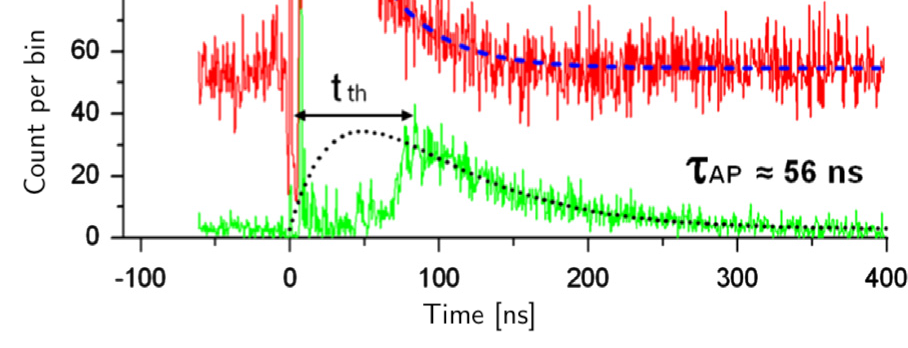
\includegraphics[width=\textwidth]{nagyap}
    
    \caption{\label{fig:nagyap} Excerpt of Figure~11 from \cite{nagy2014},
    showing the histogram of the delay of pulses successive to initial 1 PE
    pulses, selected with an upper bound on their amplitude to get afterpulses
    while removing dark count, and fitted with an exponential decay with
    constant $\tau_\text{AP}$ multiplied by the correction in
    \autoref{eq:recfactor}.}
    
\end{figure}

\cite{garutti2014} has approximately the same temporal cut and parameters, and
gets a good fit with either one or two uncorrected exponentials. We anticipate
that in our analysis the temporal cut will be even further relative to
$\tau_\text{rec}$ than in the referenced articles, so we will not be able to
discriminate the two models. For simplicity, we will keep the plain
exponentials.

The other matter with low delays is the amplitude reduction. Here all the
references we consulted agree on multiplying the 1 PE amplitude by the recharge
factor \eqref{eq:recfactor}, thus assuming that amplitude is proportional to
overvoltage. We will see this may not be accurate in our case.

Now to another topic: multiple afterpulses. The afterpulse avalanche itself
produces trapped carriers. However, since it may have smaller amplitude than a
primary avalanche, they will be less than those left around by a complete
discharge. Other two possible effects that we hypothesize, although we are not
sure about them, are: that if traps are not too far from saturation after an
avalanche, the additional afterpulses will be even more suppressed, and that an
avalanche may partially ``purge'' traps.

Keeping into account all these interactions is tedious, so we make a
simplifying assumption, inspired by the last consideration: that each avalanche
resets the cell to a fixed state. In this model, a pulse can have at most one
afterpulse. An eventual successive afterpulse must be produced by the first
afterpulse, not the initial pulse. \cite{cova1991} implicitly states that this
is not the case, although their experimental conditions are different because
the procedure they use to fill the traps is different from a ``spontaneous''
avalanche. Since these are second order effects, we anticipate that the
probabilities involved are small and that we probably would not be able to
falsify the simplified model with our data.

Bringing the DiCT model into the picture, each afterpulse will have its own
DiCT tree. We suppose that a smaller avalanche should emit less photons and
thus have less cross talk; again, for the sake of simplicity, we will assume
that the DiCT probability remains the same instead.

Since the DiCT involves separate cells, even with our ``resetting afterpulse''
model if the initial pulse has more than one PE then multiple afterpulses due
to the same initial pulse are allowed. We call this case \emph{parallel
afterpulses}, while the case with an afterpulse of an afterpulse \emph{series
afterpulses}.

\subsection{Expected values}

%         I numeri che ci aspettiamo circa di vedere (da Savarese)

\section{Data}
%         Elenco dei file con il percorso
%         Istogrammi 2D di tutti i file _2 (salto _1 perché a 5 VoV ha i doppi picchi), ricordarsi di togliere il digit 0 per non occupare il range dinamico con la saturazione
%         Controllo i trigger degli altri file
%         Doppi picchi

\marginpar{\cite[p.~2, after eq.~5]{nagy2014} says that they use a short
wavelength (blue) laser such that photons get absorbed directly in the junction
and not in the neutral region below and then diffuse. What's the situation in
LNGS? Maybe \cite{savarese2018} says something on this.}

\section{Peak finding}

\subsection{Filtering}
% il problema dei template non lineari

\subsection{Baseline}

\subsection{Laser peak}

\subsection{Other peaks}

\subsection{PE}

\subsection{Filter deconvolution}

\section{Random pulses rate}

\section{Afterpulses}
%         Spiegare per bene come faccio i fit bayesiani con minimi quadrati e cosa significa statisticamente correggere con sqrt(chi2/dof)

\section{Direct cross talk}

\subsection{Random pulses}

\subsection{Afterpulses}

\subsection{Laser pulses}

\subsection{Results}

\section{Conclusions}

% VETO
% simulazione (confronto con cosa c'è in Pyreco, dire che è quasi il nostro
% stesso modello)
% dire che i casini per delay piccoli con gli afterpulse alla fine non
% dovrebbero contare troppo perché l'ampiezza è più piccola
% scusarsi per non aver fatto gli ovvi miglioramenti: fittare con più di 1 pe
% come selezione iniziale per gli afterpulse, modellare meglio l'altezza degli
% afterpulse, studiare un modello empirico intermedio per il cross talk,
% tenere conto dei doppi picchi nei fit.
% peak finding, citare LZ:
% Conferenza dance machine learning workshop
% https://indico.physics.lbl.gov/event/1192/contributions/4934/
